% 一幅完整的生成式解剖插画：神经元1的轴突分支影响神经元2和3。
% 全部标注、引导线与传递方向由 TikZ 排版；不重复拼接单细胞素材。
\begin{tikzpicture}[x=1mm,y=1mm,font=\figurefont\footnotesize,
  leader/.style={draw=FigureMuted,line width=0.5pt},
  annotation/.style={fill=none,inner sep=0.7mm},
  transmission/.style={book arrow,draw=FigureBlue,line width=1pt}]
  \node[anchor=south west,inner sep=0pt] at (0,0)
    {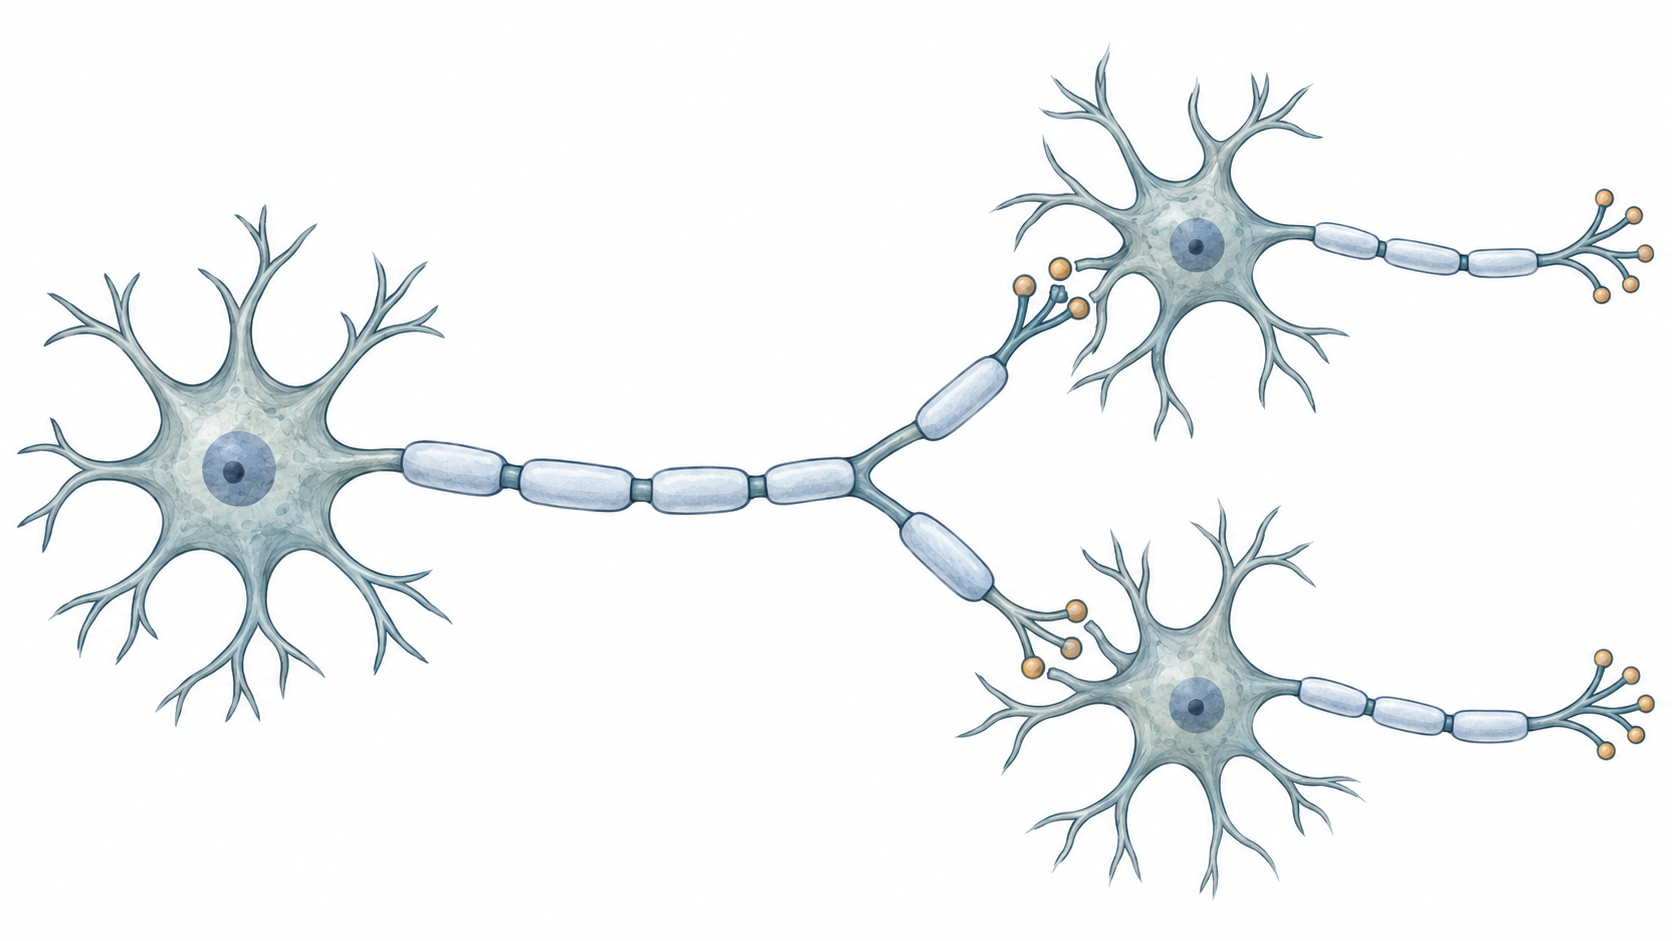
\includegraphics[width=168mm]{figures/03-models/02-neural-network-models/generated/neural-overview-neuron-divergence.png}};
  \node[annotation] at (25,86) {神经元1};
  \node[annotation] at (140,91) {神经元2};
  \node[annotation] at (142,6) {神经元3};
  \node[annotation] (dendrites) at (9,76) {树突};
  \draw[leader] (dendrites.south)--(9,70)--(11,64);
  \node[annotation] (soma) at (9,23) {胞体};
  \draw[leader] (soma.north)--(10,29)--(18,43);
  \node[annotation] (nucleus) at (35,21) {细胞核};
  \draw[leader] (nucleus.north)--(32,31)--(24,47);
  \node[annotation] (axon) at (41,64) {轴突};
  \draw[leader] (axon.south)--(41,57)--(37,48);
  \node[annotation] (myelin) at (59,65) {髓鞘};
  \draw[leader] (myelin.south)--(59,58)--(57,46);
  \node[annotation] (ranvier) at (67,26) {郎飞结};
  \draw[leader] (ranvier.north)--(67,34)--(64.4,45.3);
  \node[annotation] (branch) at (86,59) {轴突分支};
  \draw[leader] (branch.south)--(86,51)--(86,46);
  \node[annotation] (terminals) at (91,80) {轴突末梢};
  \draw[leader] (terminals.south)--(96,75)--(102.8,66);
  \node[annotation] (synapseone) at (110,53) {突触1};
  \draw[leader] (synapseone.north)--(110,60)--(107.1,67.5);
  \node[annotation] (synapsetwo) at (91,14) {突触2};
  \draw[leader] (synapsetwo.north)--(98,24)--(108.7,32.3);
  \draw[transmission] (43,53)--(77,53);
  \node[annotation,text=FigureBlue] at (61,57) {信号传递};
  \draw[transmission] (87,51) to[out=35,in=215] (98,62);
  \draw[transmission] (87,40) to[out=-35,in=155] (99,33);
\end{tikzpicture}
